\documentclass[12pt,a4paper]{article}

\usepackage[margin=1in]{geometry}
\usepackage{graphicx}
\usepackage{booktabs}
\usepackage{array}
\usepackage{float}
\usepackage{hyperref}
\usepackage{setspace}
\usepackage{titlesec}

\hypersetup{
    colorlinks=true,
    linkcolor=black,
    urlcolor=blue,
    pdftitle={End-to-End Deep Learning Pipeline for Visual Recognition},
    pdfauthor={Project Report}
}

\setstretch{1.15}
\titleformat{\section}{\large\bfseries}{\thesection}{0.75em}{}

\title{\textbf{Computer Vision Project}\\[0.5em]
\Large End-to-End Deep Learning Pipeline for Visual Recognition\\[0.3em]
\large Animal Image Classification Using Transfer Learning}
\author{
Team Members:\\[0.3em]
1. Bassant Hossam Salah Eldeen\\
2. Shahda Mohamed Abd Alkareem\\
3. Steven Ragy\\
4. Ahmed Ehab Ahmed Elattar\\
5. Eyad Hesham Ibrahim\\
6. Zeyad Wael Helmy\\
7. Basmalla Helal\\
8. Basama Ahmed\\[1em]
Under Supervision of:\\[0.3em]
eng.Habiba Atef\\
Dr.\ Shimaa Elgazar
}
\date{\today}

\begin{document}

\maketitle

\section{Introduction}
Computer vision systems depend not only on model architecture but also on disciplined data preparation, validation control, and objective testing. This project implements a complete visual recognition workflow for classifying five animal categories: cat, cow, deer, dog, and lion. The main goal is to build a reproducible deep learning pipeline that satisfies academic requirements for training, validation, and final benchmarking while also producing a working application for real-time prediction.

The implementation is based on a local codebase containing three notebooks and one deployment script:
\begin{itemize}
    \item \texttt{1\_data\_exploration.ipynb}: verifies the dataset structure and visualizes the data.
    \item \texttt{2\_model\_training.ipynb}: trains a transfer-learning model with validation monitoring.
    \item \texttt{3\_evaluation.ipynb}: evaluates the final model on unseen test data.
    \item \texttt{app.py}: provides a Gradio interface for image upload and prediction.
\end{itemize}

This makes the project not only a modeling exercise, but a full machine learning pipeline from raw data organization to interactive deployment.

\section{Dataset}
The dataset source is the Kaggle dataset \emph{Animal Image Classification -- 5 Species} by \texttt{miadul}.\footnote{\url{https://www.kaggle.com/datasets/miadul/animal-image-classification-5-species}} It contains five target classes:
\begin{itemize}
    \item Cat
    \item Cow
    \item Deer
    \item Dog
    \item Lion
\end{itemize}

In the local project, the archive was extracted into \texttt{data/animals\_dataset/} and normalized to match the final code convention:
\begin{itemize}
    \item split folders: \texttt{train}, \texttt{val}, \texttt{test}
    \item class folders: \texttt{cat}, \texttt{cow}, \texttt{deer}, \texttt{dog}, \texttt{lion}
\end{itemize}

During preprocessing, two naming inconsistencies in the archive were corrected:
\begin{itemize}
    \item \texttt{validation} was renamed to \texttt{val}
    \item \texttt{deep} was renamed to \texttt{deer}
\end{itemize}

The actual local extracted archive used in the experiments produced the following split counts:

\begin{table}[H]
\centering
\begin{tabular}{lcccccc}
\toprule
Split & Cat & Cow & Deer & Dog & Lion & Total \\
\midrule
Train & 91 & 86 & 87 & 111 & 89 & 464 \\
Validation & 17 & 15 & 17 & 17 & 17 & 83 \\
Test & 17 & 16 & 16 & 16 & 17 & 82 \\
\bottomrule
\end{tabular}
\caption{Observed image counts in the normalized local dataset.}
\end{table}

Although the Kaggle page describes a simple five-species image classification task and notes a standardized image setup, the local archive inspection showed that the images were not perfectly uniform in original dimensions. Therefore, the codebase resizes all inputs to \texttt{224 \(\times\) 224} during training, validation, testing, and deployment for consistency.

\begin{figure}[H]
    \centering
    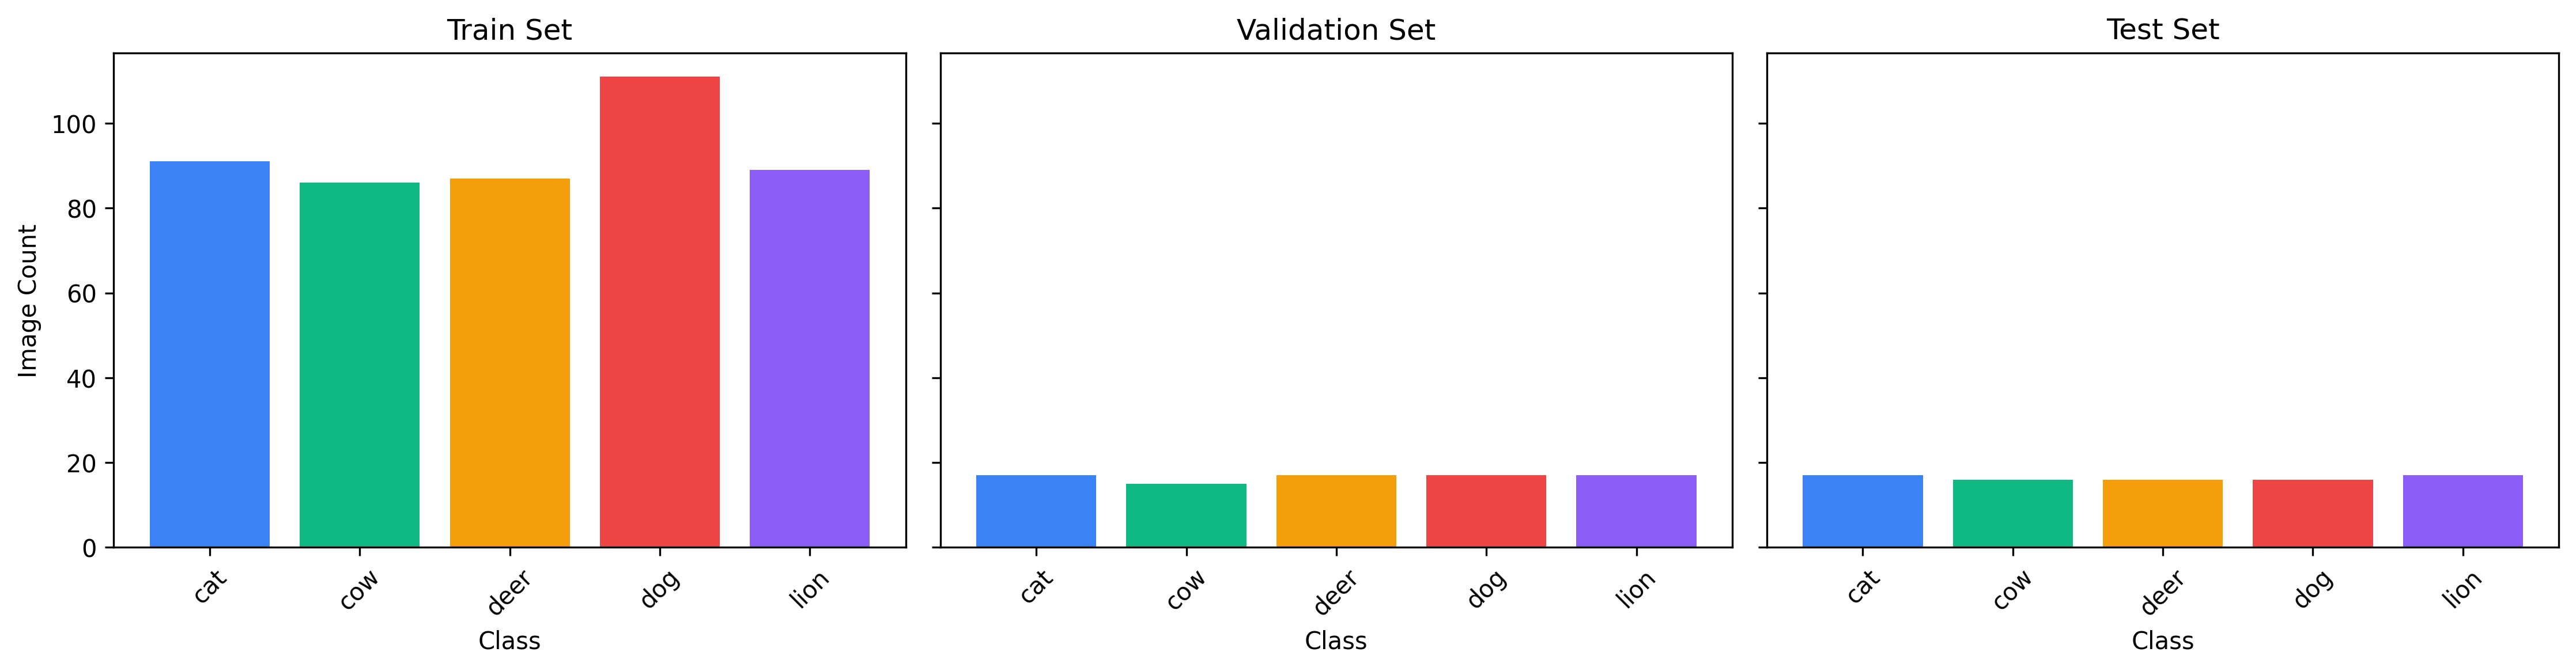
\includegraphics[width=0.88\textwidth]{imgs/class_distribution.png}
    \caption{Class distribution across the train, validation, and test splits.}
\end{figure}

\section{Methodology}
The project follows the required three-tier methodology: training, validation, and testing.

\subsection{Training Phase}
The training phase uses a convolutional neural network through transfer learning. Specifically, a pretrained ResNet18 model from \texttt{torchvision} was selected because it is lightweight, reliable, and appropriate for a small image dataset. Instead of training from scratch, the pretrained feature extractor was reused and only the final fully connected layer was replaced to match the five project classes.

The training notebook applies the following preprocessing and augmentation steps:
\begin{itemize}
    \item Resize all images to \texttt{224 \(\times\) 224}
    \item Random horizontal flipping
    \item Random rotation up to 15 degrees
    \item Color jitter for brightness, contrast, and saturation
    \item Tensor conversion
    \item Normalization using ImageNet mean and standard deviation
\end{itemize}

The model was trained using:
\begin{itemize}
    \item Batch size = 16
    \item Learning rate = 0.001
    \item Optimizer = Adam
    \item Loss function = CrossEntropyLoss
    \item Maximum epochs = 20
\end{itemize}

These settings were chosen to balance training stability, reasonable speed, and reduced overfitting on a relatively small dataset.

\subsection{Validation Phase}
The validation split was used at the end of every epoch to monitor generalization. This stage is essential because a model can appear to perform well on training data while failing on unseen data. To address that risk, the training notebook includes two control mechanisms:
\begin{itemize}
    \item \textbf{Learning-rate scheduling}: \texttt{ReduceLROnPlateau} lowers the learning rate when validation loss stops improving.
    \item \textbf{Early stopping}: training stops after several non-improving validation epochs, preventing unnecessary overfitting.
\end{itemize}

The best checkpoint is saved to \texttt{models/best\_model.pth} whenever the validation loss improves. The checkpoint stores:
\begin{itemize}
    \item model weights
    \item class names
    \item best validation loss
    \item training history
\end{itemize}

\subsection{Testing Phase}
After training was complete, the best saved checkpoint was evaluated on the unseen test split. No random augmentation was used in this phase. Test images were only resized, converted to tensors, and normalized. This keeps final benchmarking unbiased and aligned with standard evaluation practice.

The evaluation notebook computes:
\begin{itemize}
    \item confusion matrix
    \item overall accuracy
    \item precision per class
    \item recall per class
    \item F1-score per class
    \item macro and weighted averages
\end{itemize}

\begin{figure}[H]
    \centering
    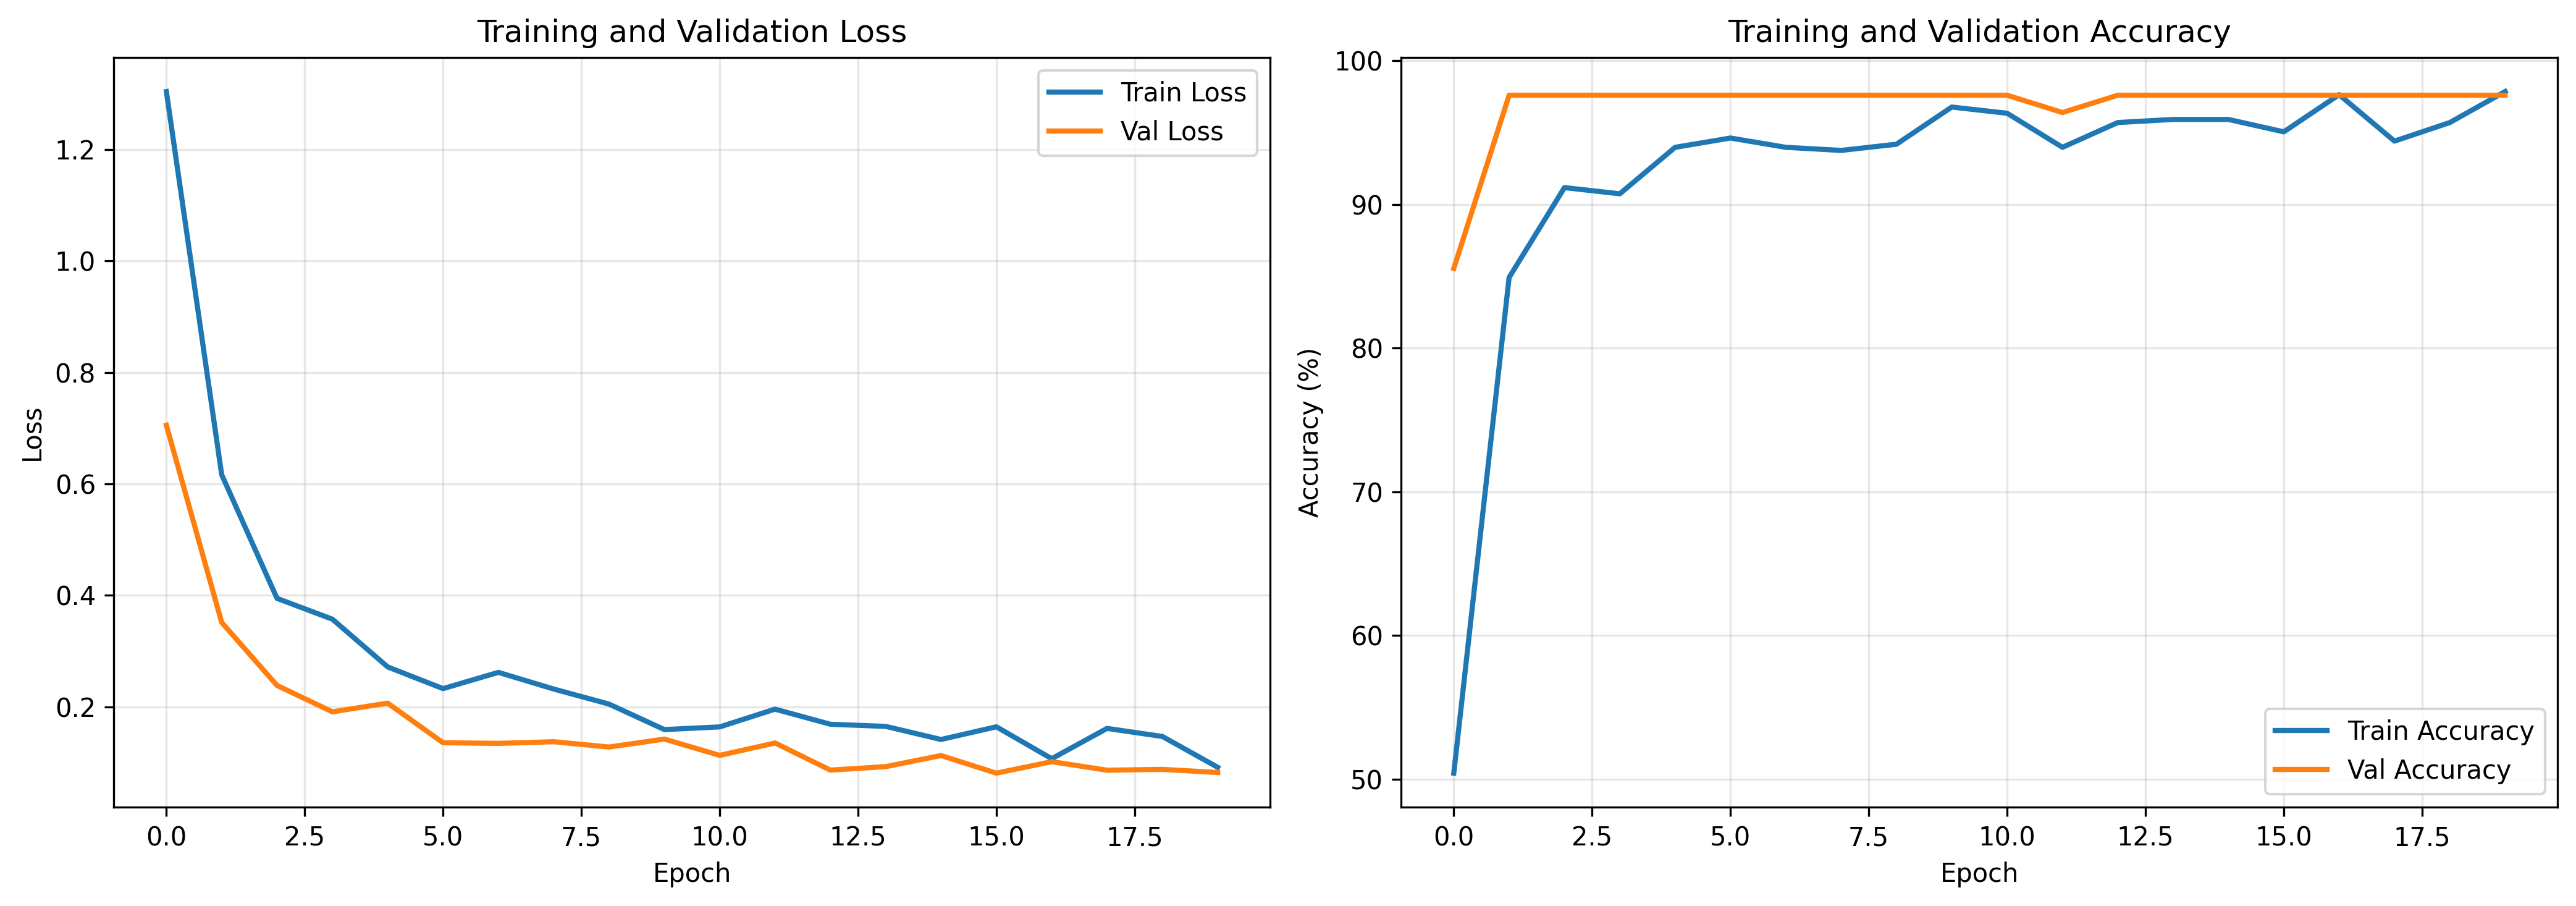
\includegraphics[width=0.9\textwidth]{imgs/training_curves.png}
    \caption{Training and validation loss/accuracy curves produced by the training notebook.}
\end{figure}

\section{Results}
The codebase produced all expected result artifacts:
\begin{itemize}
    \item \texttt{class\_distribution.png}
    \item \texttt{sample\_images.png}
    \item \texttt{training\_curves.png}
    \item \texttt{classification\_report.txt}
    \item \texttt{confusion\_matrix.png}
    \item \texttt{sample\_predictions.png}
    \item \texttt{best\_model.pth}
\end{itemize}

The final evaluation report from the local run gave:
\begin{itemize}
    \item Test accuracy = 97.56\%
    \item Macro precision = 0.9778
    \item Macro recall = 0.9765
    \item Macro F1-score = 0.9757
\end{itemize}

Per-class results are shown in Table~\ref{tab:classmetrics}.

\begin{table}[H]
\centering
\begin{tabular}{lcccc}
\toprule
Class & Precision & Recall & F1-score & Support \\
\midrule
Cat & 1.0000 & 0.8824 & 0.9375 & 17 \\
Cow & 1.0000 & 1.0000 & 1.0000 & 16 \\
Deer & 0.8889 & 1.0000 & 0.9412 & 16 \\
Dog & 1.0000 & 1.0000 & 1.0000 & 16 \\
Lion & 1.0000 & 1.0000 & 1.0000 & 17 \\
\bottomrule
\end{tabular}
\caption{Per-class performance on the unseen test split.}
\label{tab:classmetrics}
\end{table}

These metrics show excellent overall performance. Three classes achieved perfect precision and recall, while the remaining small errors appeared mainly in cat recall and deer precision. Given the relatively small test split, even one or two mistakes can noticeably affect the class-specific metrics, so these results should be interpreted as strong but still dependent on limited test data size.

\begin{figure}[H]
    \centering
    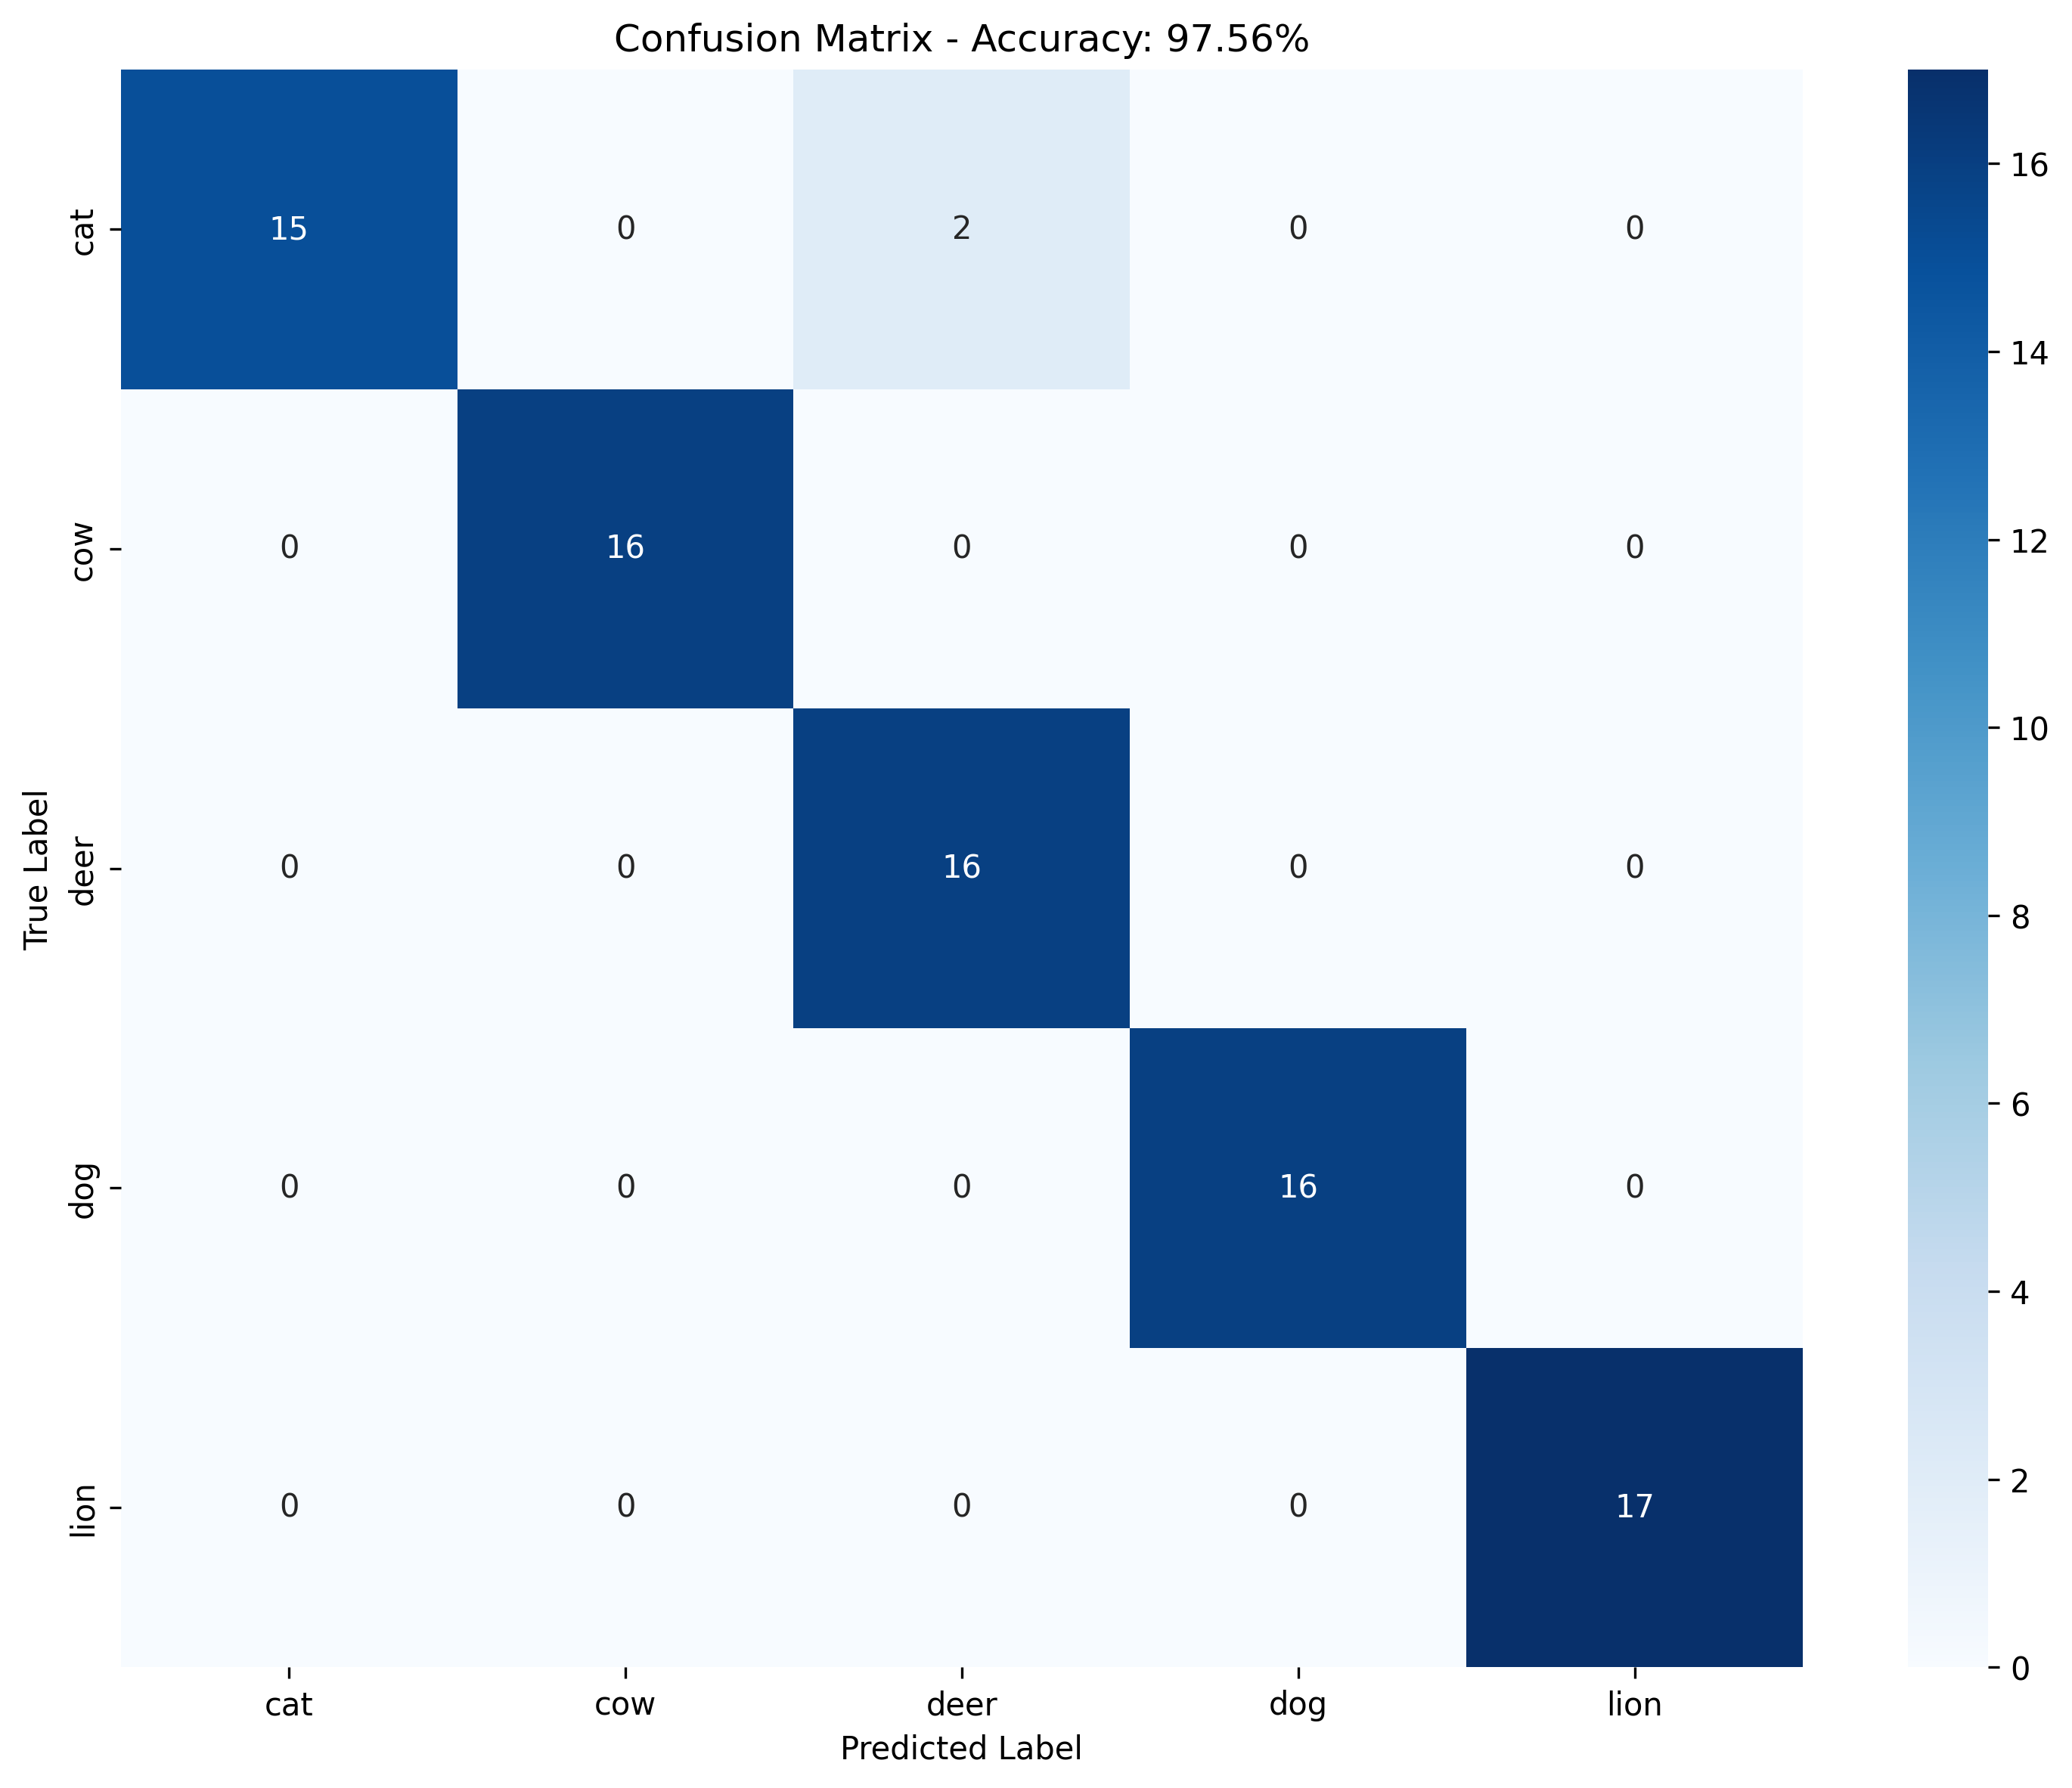
\includegraphics[width=0.78\textwidth]{imgs/confusion_matrix.png}
    \caption{Confusion matrix of the final model on the unseen test split.}
\end{figure}

\section{Review}
From a technical perspective, the project satisfies the required pipeline goals and demonstrates good software organization.

\subsection*{Strengths}
\begin{itemize}
    \item The codebase is separated into clear stages: exploration, training, evaluation, and deployment.
    \item The methodology explicitly uses training, validation, and testing as required.
    \item Transfer learning made it possible to achieve strong performance on a modest dataset.
    \item Early stopping and validation-based monitoring reduced overfitting risk.
    \item The final model is deployable through a working Gradio application.
    \item The project generates both quantitative and qualitative outputs for interpretation.
\end{itemize}

\subsection*{Limitations}
\begin{itemize}
    \item The local extracted dataset is not perfectly balanced.
    \item The test split contains only 82 images, so the final score can shift noticeably with a small number of errors.
    \item Original image sizes vary, which required resizing before modeling.
    \item Only one architecture was trained in the final pipeline, so no model comparison study was included.
\end{itemize}

\subsection*{Deployment Note}
The project also includes a Gradio application in \texttt{app/app.py}. The app reconstructs the trained ResNet18 classifier, loads the saved checkpoint, preprocesses uploaded images exactly as in evaluation, and returns the predicted class with probability scores. This demonstrates that the project is not only analytically complete but also practically usable.

\section{Conclusion}
This project successfully implemented an end-to-end deep learning pipeline for visual recognition using an animal image classification dataset. The workflow covered data verification, supervised training, validation-based optimization, final testing, and real-time deployment. The training phase learned class-discriminative visual features through a transfer-learning approach based on ResNet18. The validation phase controlled overfitting through learning-rate scheduling and early stopping. The testing phase provided an unbiased estimate of performance on unseen data using confusion matrix, accuracy, precision, recall, and F1-score.

The final model achieved 97.56\% test accuracy with consistently high class-wise performance, showing that the pipeline generalizes well to the available unseen test data. In addition to meeting the academic requirements, the project produced a clean codebase, interpretable results, and a working application suitable for demonstration.

\end{document}
